\documentclass[12pt]{article}

\usepackage{amsmath}
\numberwithin{figure}{subsection}
\numberwithin{table}{subsection}
\numberwithin{equation}{subsection}

\usepackage{array}
\usepackage{caption}
\usepackage[top=1in, bottom=1in, left=0.75in, right=0.75in]{geometry}

\usepackage{graphicx}
\graphicspath{{figures/}}

\usepackage[colorlinks=true, allcolors=blue]{hyperref}
\usepackage[utf8]{inputenc}
\usepackage{multirow}
\usepackage{pdfpages}
\usepackage[section]{placeins}

\title{ECE 271: Chapter 5 Reading Report}
\author{Phi Luu}
\date{November 14\textsuperscript{th}, 2018}

\begin{document}

\maketitle

%%%%%%%%%%%%%%%%%%%%%%%%%%%%%%%%%%%%%%%%%%%%%%%%%%%%%%%%%%%%%%%%%%%%%%%%%%%%%%%%
% Chapter Outline
%%%%%%%%%%%%%%%%%%%%%%%%%%%%%%%%%%%%%%%%%%%%%%%%%%%%%%%%%%%%%%%%%%%%%%%%%%%%%%%%
\section{Chapter Outline}

%%%%%%%%%%%%%%%%%%%%%%%%%%%%%%%%%%%%%%%%
% Introduction
%%%%%%%%%%%%%%%%%%%%%%%%%%%%%%%%%%%%%%%%
\subsection{Introduction}

Chapter 2 covers combinational logic; chapter 3 covers sequential logic; and chapter 4 covers hardware description language. This chapter puts combinational logic and sequential logic together to form digital building blocks, making larger hardware. This chapter is the transition from the lower level---logic---to the higher level---architecture.

This chapter will go through basic digital building blocks, including arithmetic circuits, counters, shift registers, memory arrays, and logic arrays. These building blocks are used to build a microprocessor.

%%%%%%%%%%%%%%%%%%%%%%%%%%%%%%%%%%%%%%%%
% Arithmetic Circuits
%%%%%%%%%%%%%%%%%%%%%%%%%%%%%%%%%%%%%%%%
\subsection{Arithmetic Circuits}

Arithmetic circuits are the central building blocks of computers. They enable computers and digital logic perform arithmetic functions, such as addition, subtraction, multiplication, division, comparisons, and shifts.

\begin{enumerate}
  %%%%%%%%%%%%%%%%%%%%
  % Addition
  %%%%%%%%%%%%%%%%%%%%
  \item \textbf{Addition}

  Addition is one of the most common operations in digital systems. The \textit{half adder} and the \textit{full adder} mentioned in earlier chapters are two of the digital building blocks that perform addition.

  \begin{enumerate}
    %%%%%%%%%%
    % Half Adder
    %%%%%%%%%%
    \item \textbf{Half Adder}

    The most basic example of a half adder is a 1-bit half adder. The half adder takes in two inputs---two binary bit---and add them together to output the sum and the carry out, as demonstrated by Figure~\ref{fig:1_bit_half_adder} below:

    \newpage

    \begin{figure}[ht]
      \centering
      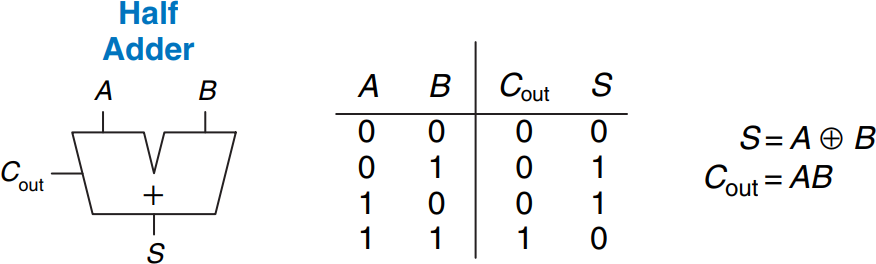
\includegraphics[width=0.75\textwidth]{half_adder_1_bit.png}
      \caption{A 1-bit half adder's block schematic, truth table, and Boolean equations (respectively)}
      \label{fig:1_bit_half_adder}
    \end{figure}

    Similar to decimal addition, binary addition "carries" a 1 to the next column (next half adder) when the result overflows---in this case, the result of $1 + 1$. Using the truth table provided in Figure~\ref{fig:1_bit_half_adder}, the Boolean equation of $S$ and $C_{out}$ can be solved as $S = A \oplus B$ (XOR logic) and $C_{out} = AB$ (AND logic).

    By putting multiple half adders together, a multi-adder system is formed. The $C_{out}$ (carry out) of the less significant bit is the carry in of the more significant bit---in other words, from right to left---just like decimal addition. However, the half adder lacks the $C_{in}$ (carry in) input. The \textit{full adder} solves this problem.

    %%%%%%%%%%
    % Full Adder
    %%%%%%%%%%
    \item \textbf{Full Adder}

    As described in the half adder section, the \textit{full adder} takes in three inputs---two binary bits $A$ and $B$ and one carry-in bit $C_{in}$---and produces two inputs, one carry-out bit $C_{out}$ and one sum bit $S$.

    \begin{figure}[ht]
      \centering
      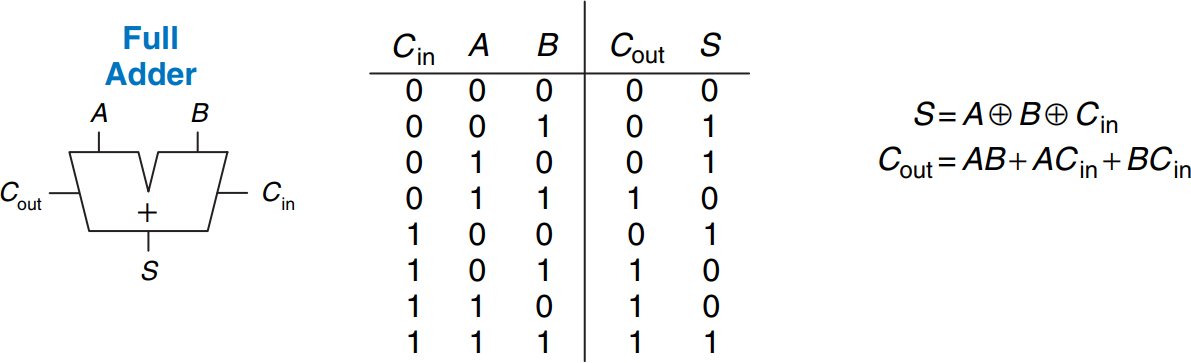
\includegraphics[width=0.75\textwidth]{full_adder_1_bit.png}
      \caption{A 1-bit full adder's block schematic, truth table, and Boolean equations (respectively)}
      \label{fig:1_bit_full_adder}
    \end{figure}

    The addition of the full adder is exactly like that of the half adder, but the full adder takes in an extra carry-in bit and adds three 1-bit binary numbers $A$, $B$, and $C_{in}$. Using Boolean simplification methods (K-maps or pure Boolean algebra), the Boolean equations of the sum $S$ and the carry out $C_{out}$ can be expressed by Figure~\ref{fig:1_bit_full_adder}. Knowing the Boolean equations, the designer can easily implement the half adder and the full adder using combinational logic.

    %%%%%%%%%%
    % Carry Propagate Adder
    %%%%%%%%%%
    \item \textbf{Carry Propagate Adder}

    An $N$-bit adder sums two $N$-bit inputs, $A$ and $B$, and a carry in $C_{in}$ to produce an $N$-bit result $S$ and a carry out $C_{out}$. The \textit{carry propagate adder} propagates the carry out of one bit to the next. The block schematic of the carry propagate adder is similar to that of the full adder, but the carry propagate adder takes in $N$-bit inputs instead of 1-bit, as illustrated by Figure~\ref{fig:carry_propagate_adder} below:

    \begin{figure}[ht]
      \centering
      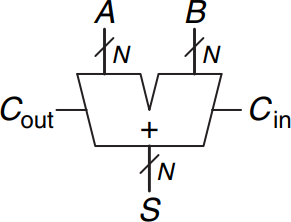
\includegraphics[width=0.25\textwidth]{carry_propagate_adder.png}
      \caption{A carry propagate adder's block schematic}
      \label{fig:carry_propagate_adder}
    \end{figure}

    %%%%%%%%%%
    % Ripple-Carry Adder
    %%%%%%%%%%
    \item \textbf{Ripple-Carry Adder}

    The simplest way to build an $N$-bit carry propagate adder is to chain together $N$ full adders. As stated in the full adder section, the $C_{out}$ of the less significant bit is the $C_{in}$ of the more significant bit (carrying from right to left). This is called the \textit{ripple-carry adder}. The advantage of this system is its simplicity---a large system can be built by chaining multiple identical modules. However, its disadvantage is its speed---as $C_N$ depends on $C_{N - 1}$, which depends on $C_{N - 2}$, which depends on $C_{N - 3}$, and so on until $C_0$. The block schematic of a 32-bit ripple-carry adder is as illustrated by Figure~\ref{fig:ripple_carry_adder} below:

    \begin{figure}[ht]
      \centering
      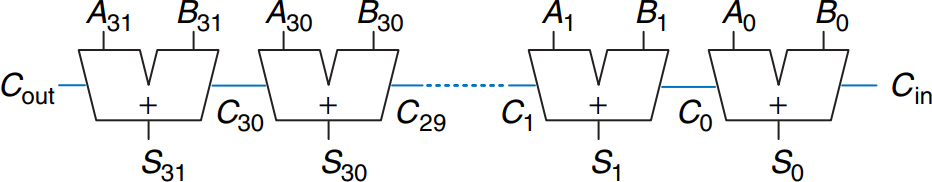
\includegraphics[width=0.75\textwidth]{ripple_carry_adder.png}
      \caption{A ripple-carry adder's block schematic}
      \label{fig:ripple_carry_adder}
    \end{figure}

    The delay of the adder, $t_{ripple}$, grows linearly with the number of bits, as given in Equation~\ref{eq:ripple_carry_adder_delay}, where $t_{FA}$ is the delay of a full adder:

    \begin{equation} \label{eq:ripple_carry_adder_delay}
      t_{ripple} = N t_{FA}
    \end{equation}

    %%%%%%%%%%
    % Carry-Lookahead Adder
    %%%%%%%%%%
    \item \textbf{Carry-Lookahead Adder}

    The \textit{carry-lookahead adder} solves the ripple-carry adder by dividing the adder into \textit{blocks} and providing circuitry to quickly determine the carry out of a block as soon as the carry in is known. It \textit{looks ahead} across the blocks rather than waiting to ripple through all the full adders inside a block. For example, a 32-bit adder can be divided into eight 4-bit blocks.

    Carry-lookahead adders use \textit{generate} (G) and \textit{propagate} (P) signals that describe how a column or block determines the carry out.

    The $i$th column of an adder \textit{generates} a carry if it produces a carry out regardless of the value of the carry in. According to the truth table in Figure~\ref{fig:1_bit_full_adder}, $C_{out} = 1$ regardless of the value of $C_{in}$ if and only if $A = B = 1$. Thus, $G_i = A_i B_i$ in the $i$th column of the an adder.

    The $i$th column is said to \textit{propagate} a carry if it produces a carry out whenever there is a carry in. Using Figure~\ref{fig:1_bit_full_adder} once again, $C_{out} = 1$ when $C_{in} = 1$ if and only if $A = 1$ or $B = 1$. Thus, $P_i = A_i + B_i$.

    Putting $G_i$ and $P_i$ together, the $i$th column of an adder will generate a carry out $C_i$ if either generates a carry, $G_i$, or propagates a carry in, $P_i C_{i - 1}$. In equation form,

    \begin{equation}
      C_i = A_i B_i + \left( A_i + B_i \right) C_{i - 1} =  G_i + P_i C_{i - 1}
    \end{equation}

    Using the block generate and propagate signals, the carry out of the block, $C_i$ can be computed by the carry in to the block, $C_j$,

    \begin{equation}
      C_i = G_{i:j} + P_{i:j} C_j
    \end{equation}

    The delay of an $N$-bit adder divided into $k$-bit block is as follows:

    \begin{equation}
      t_{CLA} = t_{pg} + t_{pg\_block} + \left( \frac{N}{k} - 1 \right) t_{AND\_OR} + kt_{FA}
    \end{equation}

    %%%%%%%%%%
    % Prefix Adder
    %%%%%%%%%%
    \item \textbf{Prefix Adder}

    \textit{Prefix adders} extend the generate and propagate logic of the carry-lookahead adder to perform addition even faster. The strategy of the prefix adder is to compute the carry in $C_{i - 1}$ for each column $i$ as fast as possible, then to compute the sum using

    \begin{equation} \label{equation:1.2.5}
      S_i = \left( A_i \oplus B_i \right) \oplus C_{i - 1}
    \end{equation}

    The delay of an $N$-bit prefix adder is

    \begin{equation} \label{equation:1.2.6}
      t_{PA} = t_{pg} + \log_2{N \left( t_{pg\_prefix} \right)} + t_{XOR}
    \end{equation}
  \end{enumerate}

  %%%%%%%%%%%%%%%%%%%%
  % Subtraction
  %%%%%%%%%%%%%%%%%%%%
  \item \textbf{Subtraction}

  Subtraction is just a form of addition where a number adds to a negative number. Mathematically, in decimal system, $A - B = A + \left( -B \right)$.

  In binary system, to compute $Y = A - B$, first create the two's complement of $B$: invert the bits of $B$ to obtain $\overline{B}$ and add 1 to get $-B = \overline{B} + 1$. Hence, $Y = A - B = A + \overline{B} + 1$. This sum can be performed with a single carry propagate adder adding $A$ and $\overline{B}$ with $C_{in} = 1$.

  %%%%%%%%%%%%%%%%%%%%
  % Comparators
  %%%%%%%%%%%%%%%%%%%%
  \item \textbf{Comparators}

  A \textit{comparator} determines whether a binary number is equal, greater than, or less than another binary number. A comparator receives two $N$-bit binary numbers $A$ and $B$. There are two common types of comparators:

  \begin{enumerate}
    \item An \textit{equality comparator} produces a single output indicating whether $A$ is equal to $B$. A 4-bit equality comparator is illustrated by Figure~\ref{fig:4_bit_equality_comparator} below.
      \begin{figure}[ht]
        \centering
        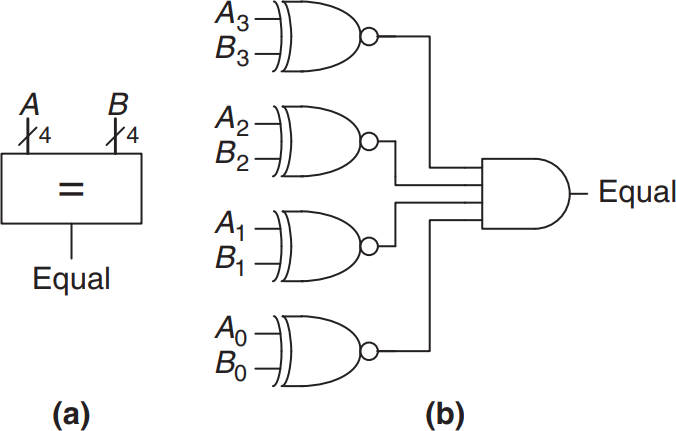
\includegraphics[width=0.5\textwidth]{equality_comparator_4_bits.png}
        \caption{A 4-bit equality comparator's (a) symbol and (b) schematic}
        \label{fig:4_bit_equality_comparator}
      \end{figure}
    \item A \textit{magnitude comparator} produces one or more outputs indicating the relative values of $A$ and $B$. It checks whether the corresponding bits in each column of $A$ and $B$ are equal using XOR gates. The numbers are equal if all of the columns are equal. Figure~\ref{fig:n_bit_magnitude_comparator} shows the symbol of an $N$-bit magnitude comparator.
      \begin{figure}[ht]
        \centering
        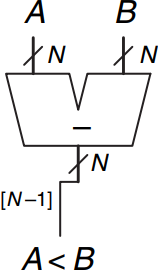
\includegraphics[width=0.125\textwidth]{magnitude_comparator_n_bits.png}
        \caption{An $N$-bit magnitude comparator}
        \label{fig:n_bit_magnitude_comparator}
      \end{figure}
  \end{enumerate}

  %%%%%%%%%%%%%%%%%%%%
  % ALU
  %%%%%%%%%%%%%%%%%%%%
  \item \textbf{ALU}

  \textit{Arithmetic/Logical Unit} (\textit{ALU}) combines a variety of mathematical and logical operations into a single unit. For example, a typical ALU might perform addition, subtraction, magnitude comparison, AND, and OR operations. The ALU forms the heart of most computer systems.

  Figure~\ref{fig:alu_symbol_and_operations} shows the symbol for an $N$-bit ALU with $N$-bit inputs and outputs. The ALU also receives a control signal $F$ that specifies which function to perform.

  \newpage

  \begin{figure}[ht]
    \centering
    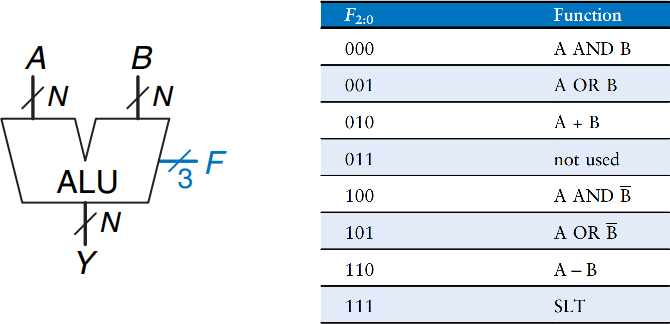
\includegraphics[width=0.75\textwidth]{alu_symbol_and_operations.png}
    \caption{An ALU's symbol and operations}
    \label{fig:alu_symbol_and_operations}
  \end{figure}

  %%%%%%%%%%%%%%%%%%%%
  % Shifters and Rotators
  %%%%%%%%%%%%%%%%%%%%
  \item \textbf{Shifters and Rotators}

  \textit{Shifters} and \textit{rotators} move bits and multiply or divide by powers of 2. Shifters shift a binary number left or right by a specified number of steps. \textit{Logical shifter} and \textit{Arithmetic shifter} are two common used shifters:

  \begin{enumerate}
    \item Logical shifter shifts the number to the left (LSL) or right (LSR) and fills empty spots with 0's. For example, $11001 \text{ LSR } 2 = 00110$; $11001 \text{ LSL } 2 = 00100$.
    \item Arithmetic shifter works similarly to the logical shifter, but \textbf{on right shifts fills the most significant bits with the copy of the old most significant bit (MSB)}. This is useful for multiplying and dividing signed numbers. \textbf{Arithmetic shift left is the same as logical shift left}. For example, $11001 \text{ ASR } 2 = 11110$; $11001 \text{ ASL } 2 = 00100$.
  \end{enumerate}

  Rotators rotate number in circle such that empty spots are filled with bits shifted off the other end. For example, $11001 \text{ ROR } 2 = 01110$; $11001 \text{ ROL } 2 = 00111$.

  The operators $<<$, $>>$, and $>>>$ indicate shift left, logical shift right, and arithmetic shift right, respectively. An $N$-bit shifter can be built from $N$ $N\text{:}1$ multiplexer.

  A left shift is a special case of multiplication: \textbf{a left shift by} $\mathbf{N}$ \textbf{bits multiplies the number by} $\mathbf{2^N}$. For example, $000011_2 << 4 = 110000_2$ is equivalent to $3_{10} \cdot 2^4 = 48_{10}$.

  An arithmetic right shift is a special case of division: \textbf{an arithmetic right shift by} $\mathbf{N}$ \textbf{bits divides the number by} $\mathbf{2^N}$. For example, $11100_2 >>> 2 = 11111_2$ is equivalent to $-4_{10} \div 2^2 = -1_{10}$.

  %%%%%%%%%%%%%%%%%%%%
  % Multiplication
  %%%%%%%%%%%%%%%%%%%%
  \item \textbf{Multiplication}

  Multiplication of binary numbers is similar to decimal multiplication but involves only 0's and 1's. The \textit{partial products} are formed by multiplying a single digit of the multiplier with the entire multiplicand, as illustrated by Figure~\ref{fig:decimal_vs_binary_multiplication}.

  \newpage

  \begin{figure}[ht]
    \centering
    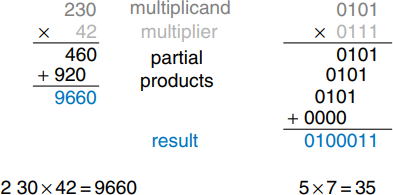
\includegraphics[width=0.5\textwidth]{decimal_vs_binary_multiplication.png}
    \caption{Decimal and binary multiplications are performed in the same way}
    \label{fig:decimal_vs_binary_multiplication}
  \end{figure}

  %%%%%%%%%%%%%%%%%%%%
  % Division
  %%%%%%%%%%%%%%%%%%%%
  \item \textbf{Division}

  Binary division can be performed using the following algorithm for $N$-bit unsigned numbers in range $\left[ 0, 2^{N - 1} \right]$:

  \begin{figure}[ht]
    \centering
    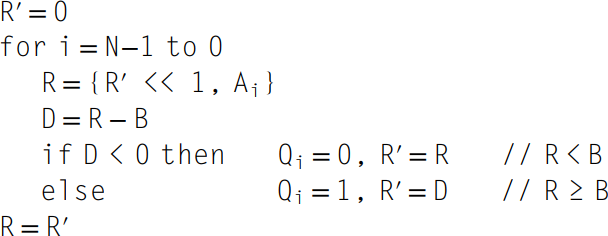
\includegraphics[width=0.5\textwidth]{division_algorithm.png}
  \end{figure}

  The \textit{partial remainder} $R$ is initialized to 0. The most significant bit of the dividend $A$ then becomes the least significant bit of $R$. The divisor $B$ is repeatedly subtracted from this partial remainder to determine whether it fits. If the difference $D$ is negative (i.e. the sign bit of $D$ is 1), then the quotient bit $Q_i$ is 0 and the difference is discarded. Otherwise, $Q_i$ is 1, and the partial remainder is updated to be the difference. In any event, the partial remainder is then doubled (left-shifted by one column), the next most significant bit of $A$ becomes the least significant bit of $R$, and the process repeats. The result satisfies $\frac{A}{B} = Q + \frac{R}{B}$.
\end{enumerate}

%%%%%%%%%%%%%%%%%%%%%%%%%%%%%%%%%%%%%%%%
% Number Systems
%%%%%%%%%%%%%%%%%%%%%%%%%%%%%%%%%%%%%%%%
\subsection{Number Systems}

Computers operate not only on unsigned and signed integers but also on fixed- and floating-point numbers that represent non-integers.

\begin{enumerate}
  %%%%%%%%%%%%%%%%%%%%
  % Fixed-Point Number Systems
  %%%%%%%%%%%%%%%%%%%%
  \item \textbf{Fixed-Point Number Systems}

  \textit{Fixed-point notation} has an implied \textit{binary point} between the integer and fraction bits, analogous to the decimal point between the integer and fraction digits of an ordinary decimal number. The implied binary point usually divides the binary number into two equal chunk of bits. The more significant chunk (the chunk on the left) can be converted to decimal using powers of 2 with positive exponent.. Conversely, the less significant chunk (the chunk on the right) can be converted to decimal using powers of 2 with negative exponents. Figure~\ref{fig:fixed_point_notation_example} shows a conversion process of a 8-bit fixed-point binary number to a decimal real number.

  \begin{figure}[ht]
    \centering
    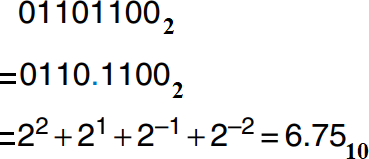
\includegraphics[width=0.4\textwidth]{fixed_point_notation_example.png}
    \caption{Fixed-point notation of 6.75 with four integer bits and four fraction bits}
    \label{fig:fixed_point_notation_example}
  \end{figure}

  Signed fixed-point numbers works for both two's complement or sign/magnitude notation. In sign/magnitude form, the most significant bit is used to indicate the sign. The two's complement representation is formed by inverting the bits of the absolute value and adding a 1 to the least significant (rightmost) bit. In the example in Figure~\ref{fig:fixed_point_notation_example}, the least significant bit position is in the $2^{-4}$ column.

  %%%%%%%%%%%%%%%%%%%%
  % Floating-Point Number Systems
  %%%%%%%%%%%%%%%%%%%%
  \item \textbf{Floating-Point Number Systems}

  Floating-point numbers are analogous to scientific notation. They overcome the limitation of having a constant number of integer and fractional bits, allowing the representation of very large and very small numbers. Like scientific notation, floating-point numbers have a \textit{sign}, \textit{mantissa} (M), \textit{base} (B), and \textit{exponent} (E). For example, the number $4.1 \times 10^3$ is the decimal scientific notation for $4100$. It has a mantissa of $4.1$, a base of $10$, and an exponent of $3$. 32 bits can be used to represent 1 sign bit, 8 exponent bits, and 23 mantissa bits.

  The IEEE floating-point standard has special cases to represent 0 (zero), $\pm \infty$ (positive and negative infinity), and NaN (Not a Number), as showed in Table~\ref{tab:ieee_floating_point_special_notations}

  \begin{table}[ht]
    \centering
    \begin{tabular}{ | c | c | c | c | }
    \hline
    \textbf{Number} & \textbf{Sign} & \textbf{Exponent} & \textbf{Fraction}       \\ \hline
    0               & X             & 00000000          & 00000000000000000000000 \\ \hline
    $\infty$        & 0             & 11111111          & 00000000000000000000000 \\ \hline
    $- \infty$      & 1             & 11111111          & 00000000000000000000000 \\ \hline
    NaN             & X             & 11111111          & Non-zero                \\ \hline
    \end{tabular}
    \caption{IEEE 754 floating-point notations for 0, $\pm \infty$, and NaN}
    \label{tab:ieee_floating_point_special_notations}
  \end{table}

  A typical 32-bit floating-point number has 1 sign bit, 8 exponent bits, and 23 fraction bits. This is called the single-precision format. There is also another format, called the \textit{double-precision floating-point format},(or \textit{doubles}) which effectively provides a greater precision and greater range:

  \begin{table}[ht]
    \centering
    \begin{tabular}{ | c | c | c | c | c | }
    \hline
    \textbf{Format} & \textbf{Total Bits} & \textbf{Sign Bits} & \textbf{Exponent Bits} & \textbf{Fraction Bits} \\ \hline
    single          & 32                  & 1                  & 8                      & 23                     \\ \hline
    double          & 64                  & 1                  & 11                     & 52                     \\ \hline
    \end{tabular}
    \caption{Single- and double-precision floating-point formats}
  \end{table}

  To add two floating-point numbers, follow these steps:

  \begin{enumerate}
    \item Extract exponent and fraction bits
    \item Prepend leading 1 to form the mantissa
    \item Compare exponent
    \item Shift smaller mantissa if necessary
    \item Add mantissas
    \item Normalize mantissa and adjust exponent if necessary
    \item Round result
    \item Assemble exponent and fraction back into floating-point number
  \end{enumerate}
\end{enumerate}

%%%%%%%%%%%%%%%%%%%%%%%%%%%%%%%%%%%%%%%%
% Sequential Building Blocks
%%%%%%%%%%%%%%%%%%%%%%%%%%%%%%%%%%%%%%%%
\subsection{Sequential Building Blocks}

\begin{enumerate}
  %%%%%%%%%%%%%%%%%%%%
  % Counters
  %%%%%%%%%%%%%%%%%%%%
  \item \textbf{Counters}

  An $N$-bit \textit{binary counter}, shown in Figure~\ref{fig:n_bit_counter_symbol_schematic}, is a sequential arithmetic circuit with clock and reset inputs and an $N$-bit output $Q$.

  \begin{figure}[ht]
    \centering
    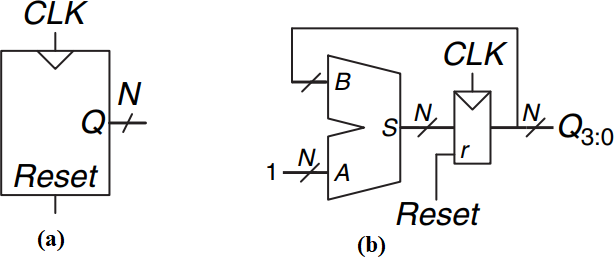
\includegraphics[width=0.5\textwidth]{counter_symbol_schematic_n_bits.png}
    \caption{An $N$-bit counter's (a) symbol and (b) schematic}
    \label{fig:n_bit_counter_symbol_schematic}
  \end{figure}

  The reset initializes the output to 0. The counter then loops through all $2^N$ possible outputs in binary order, incrementing on every rising edge of the clock.

  %%%%%%%%%%%%%%%%%%%%
  % Shift Registers
  %%%%%%%%%%%%%%%%%%%%
  \item \textbf{Shift Registers}

  A \textit{shift register} has a clock, a serial input $S_{in}$, a serial output $S_{out}$, and $N$ parallel outputs $Q_{N - 1 \text{:} 0}$, as shown in Figure~\ref{fig:shift_register_symbol_schematic}.

  \begin{figure}[ht]
    \centering
    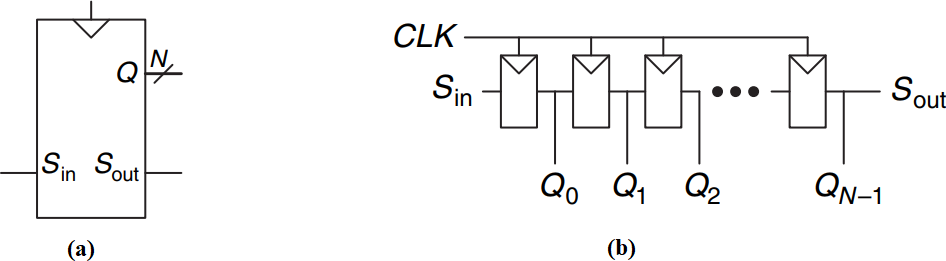
\includegraphics[width=0.75\textwidth]{shift_register_symbol_schematic.png}
    \caption{A shift register's (a) symbol and (b) schematic}
    \label{fig:shift_register_symbol_schematic}
  \end{figure}

  A shift register can be constructed from $N$ flip-flops connected in series. Some shift registers also have a reset signal to initialize the flip-flops.
\end{enumerate}

%%%%%%%%%%%%%%%%%%%%%%%%%%%%%%%%%%%%%%%%
% Memory Arrays
%%%%%%%%%%%%%%%%%%%%%%%%%%%%%%%%%%%%%%%%
\subsection{Memory Arrays}

The previous subsection introduced arithmetic and sequential circuits for manipulating data. Digital systems also require \textit{memories} to store the data used and generated by such circuits. For instance, registers built from flip-flops are a kind of memory that stores small amounts of data. This subsection describes \textit{memory arrays} that can efficiently store large amounts of information.

\begin{enumerate}
  %%%%%%%%%%%%%%%%%%%%
  % Overview
  %%%%%%%%%%%%%%%%%%%%
  \item \textbf{Overview}

  The memory is organized as a two-dimensional arry of memory cells. The memory reads or writes the contents of one of the rows of the arry. This row is specified by an \textit{Address}. The value read or written is called \textit{Data}. Each row of data is called a \textit{word}. An array with $N$-bit addresses and $M$-bit data has $2^N$ rows and $M$ columns and $2^N$ $M$-bit words. Figure~\ref{fig:generic_memory_array_symbol} shows a generic symbol for a memory array with $N$ address bits and $M$ data bits.

  \begin{figure}[ht]
    \centering
    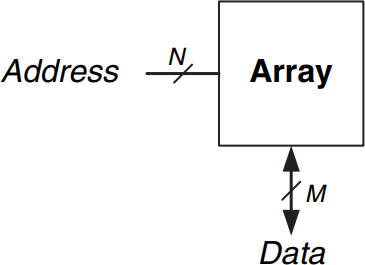
\includegraphics[width=0.25\textwidth]{generic_memory_array_symbol.png}
    \caption{Generic memory array symbol}
    \label{fig:generic_memory_array_symbol}
  \end{figure}

  The \textit{depth} of an array is the number of rows, and the \textit{width} is the number of columns, also called the word size. The size of an array is given by $depth \times width$.

  \begin{enumerate}
    %%%%%%%%%%
    % Bit Cells
    %%%%%%%%%%
    \item \textbf{Bit Cells}

    \textit{Bit cells} are the fundamental building blocks of memory arrays. Each bit cell stores 1 bit of data. Figure~\ref{fig:bit_cell} shows that each bit cell is connected to a \textit{wordline} and a \textit{bitline}.

    \begin{figure}[ht]
      \centering
      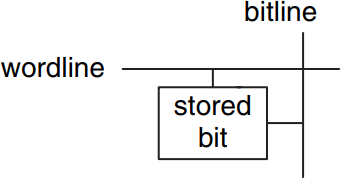
\includegraphics[width=0.25\textwidth]{bit_cell.png}
      \caption{A bit cell}
      \label{fig:bit_cell}
    \end{figure}

    For each combination of address bits, the memory asserts a single wordline that activates the bit cells in that row. If the wordline is HIGH, the stored bit transfers to or from the bitline; otherwise, the bitline is disconnected from the bit cell.

    To read a bit cell, the bitline is intially floating (Z). Then, the wordline is turned ON, allowing the stored value to drive the bitline to 0 or 1.

    To write a bit cell, the bitline is strongly driven to the desired value. Then, the worline is turned ON, connecting the bitline to the stored bit, which effectively writes the desired value to the bit cell.

    %%%%%%%%%%
    % Organization
    %%%%%%%%%%
    \item \textbf{Organization}

    Figure~\ref{fig:4x3_memory_array_symbol_function} shows the symbol and the function of a $4 \times 3$ memory array. Figure~\ref{fig:4x3_memory_array_organization} shows the internal organization of this memory array.

    \begin{figure}[ht]
      \centering
      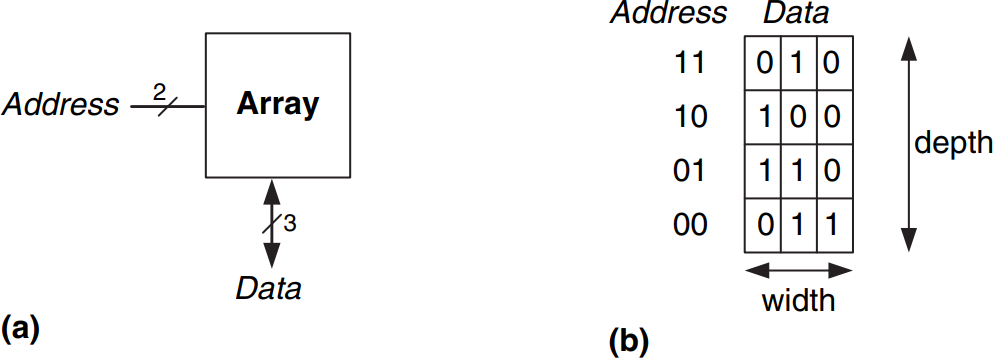
\includegraphics[width=0.5\textwidth]{memory_array_4x3_symbol_function.png}
      \caption{A $4 \times 3$ memory array's (a) symbol and (b) function}
      \label{fig:4x3_memory_array_symbol_function}
    \end{figure}

    \begin{figure}[ht]
      \centering
      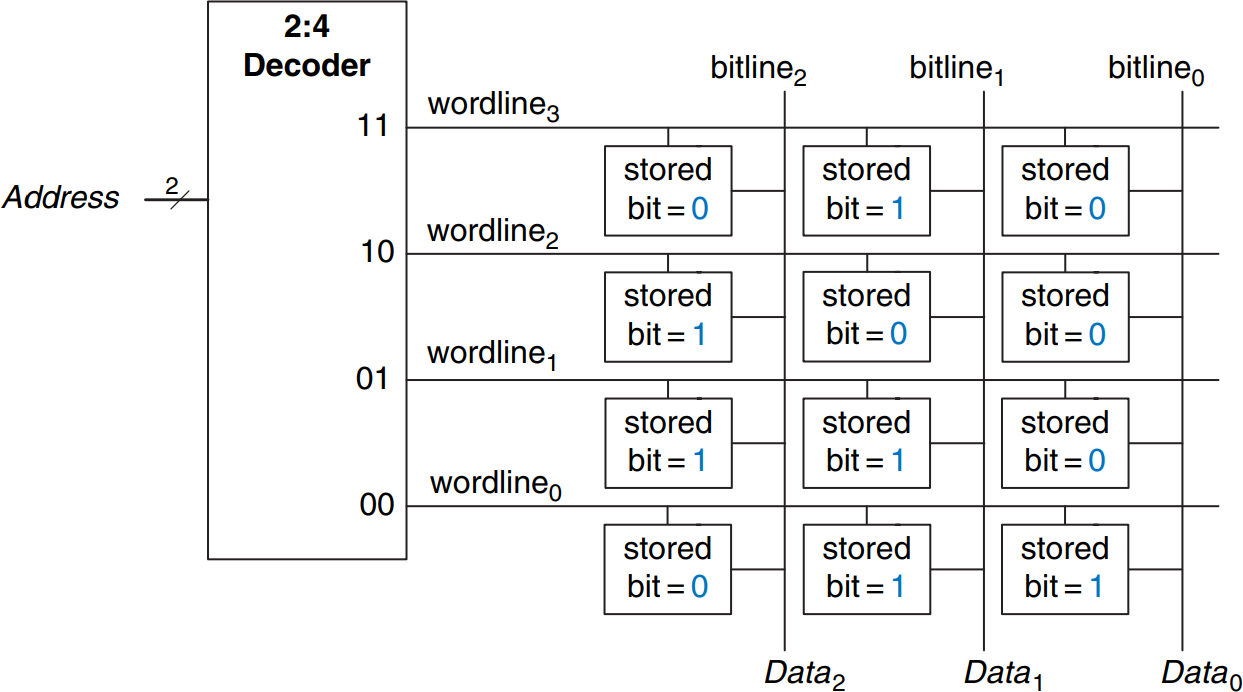
\includegraphics[width=0.75\textwidth]{memory_array_4x3_organization.png}
      \caption{A $4 \times 3$ memory array's organization}
      \label{fig:4x3_memory_array_organization}
    \end{figure}

    The organization of memory array---in this case, a $4 \times 3$ memory array---is quite easy to understand: for each wordline from the most significant bit (top) to the least significant bit (bottom), there is an array of bit cells, each connected to a bitline from the most significant bit (left) to the least significant bit (right).

    \textbf{During a memory read, a wordline is asserted, and the corresponding row of bit cells drives the bitline HIGH or LOW. During a memory write, the bitlines are driven HIGH or LOW first, and then a wordline is asserted, allowing the bitline values to be stored in that row of bitcells.}

    Using Figure~\ref{fig:4x3_memory_array_organization} for examples. To read data from \textit{Address} 10, the bitlines are first floating; the decoder asserts $\text{wordline}_2$, and the data stored inside the bitcells reads out onto the corresponding \textit{Data} bitlines: $100$. To write, say, the value $001$ to \textit{Address 11}, $\text{bitline}_2$, $\text{bitline}_1$, and $\text{bitline}_0$ are driven to $0$, $0$, and $1$, respectively; $\text{wordline}_3$ is then asserted, and the values from the bitlines are written into the corresponding bitcells.

    %%%%%%%%%%
    % Memory Ports
    %%%%%%%%%%
    \item \textbf{Memory Ports}

    \textit{Memory ports} are parts of memories which gives read and/or write access to one memory address.

    \textit{Multiported} memories can access several addresses simultaneously.

    %%%%%%%%%%
    % Memory Types
    %%%%%%%%%%
    \item \textbf{Memory Types}

    \textit{Memory types} are specified by their size ($depth \times width$) and the number and type of ports. Memories are classified based on how they store bits in the bit cell. The following list classifies the broadest types of memory and briefly how they work.

    \begin{itemize}
      \item \textbf{Random access memory (RAM)} is \textit{volatile}. Loses data without power.
        \begin{itemize}
          \item \textit{Dynamic RAM (DRAM)} stores data as a charge on a capacitor.
          \item \textit{Static RAM (SRAM)} stores data using a pair of cross-coupled inverters.
        \end{itemize}
      \item \textbf{Read only memory (ROM)} is \textit{nonvolatile}. Retains data indefinitely even without power.
    \end{itemize}
  \end{enumerate}

  %%%%%%%%%%%%%%%%%%%%
  % Dynamic Random Access Memory (DRAM)
  %%%%%%%%%%%%%%%%%%%%
  \item \textbf{Dynamic Random Access Memory (DRAM)}

  \textit{Dynamic RAM} (\textit{DRAM}) stores a bit as the presence or absence of a charge on a capacitor. Figure~\ref{fig:dram_bit_cell} shows a DRAM bit cell. The bit is stored on a capacitor. The nMOS transistor acts like a switch that either connects or disconnects the capacitor from the bitline. When the wordline is asserted, the nMOS transistor turns ON, and the stored bit value transfers to or from the bitline.

  \begin{figure}[ht]
    \centering
    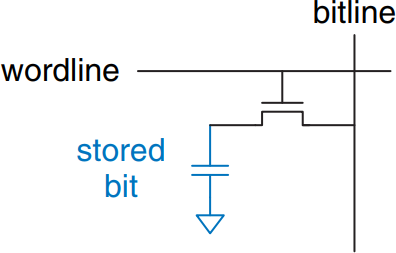
\includegraphics[width=0.4\textwidth]{dram_bit_cell.png}
    \caption{A DRAM bit cell}
    \label{fig:dram_bit_cell}
  \end{figure}

  Like a generic memory array, upon a read, data values are transferred from the capacitor to the bitline; upon a write, data values are transferred from the bitline to the capacitor.

  Reading destroys the bit value stored on the capacitor, so the data word must be restored (rewritten) after each read. Even when DRAM is not read, the contents must be refreshed (read and rewritten) every few milliseconds, because the charge on the capacitor gradually leaks away.

  %%%%%%%%%%%%%%%%%%%%
  % Static Random Access Memory (SRAM)
  %%%%%%%%%%%%%%%%%%%%
  \item \textbf{Static Random Access Memory (SRAM)}

  \textit{Static RAM} (\textit{SRAM}) is static because stored bits do not need to be refreshed. SRAM stores data on a cross-coupled inverters, as shown in Figure~\ref{fig:sram_bit_cell} below:

  \begin{figure}[ht]
    \centering
    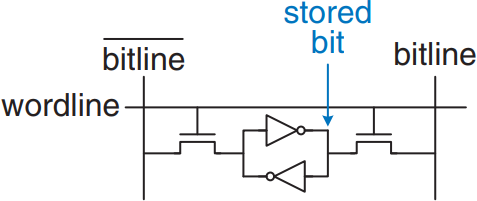
\includegraphics[width=0.4\textwidth]{sram_bit_cell.png}
    \caption{A SRAM bit cell}
    \label{fig:sram_bit_cell}
  \end{figure}

  Each cell has two outputs, bitline and $\overline{\text{bitline}}$. When wordline is asserted, both nMOS transistors turn on, and the data is transferred to or from the bitlines. Unline DRAM, the cross-coupled inverters restore the value of the stored bit.

  %%%%%%%%%%%%%%%%%%%%
  % Area and Delay
  %%%%%%%%%%%%%%%%%%%%
  \item \textbf{Area and Delay}

  Flip-flops, DRAM, and SRAM are all volatile memories, but each has different area and delay characteristics. Table~\ref{tab:memory_comparison} compares these three types of memory.

  \begin{table}[ht]
    \centering
    \begin{tabular}{ | c | c | c | }
    \hline
    \textbf{Memory Type} & \textbf{Transistors per Bit Cell} & \textbf{Latency} \\ \hline
    Flip-flop            & $\approx 20$                      & Fast             \\ \hline
    SRAM                 & 6                                 & Medium           \\ \hline
    DRAM                 & 1                                 & Slow             \\ \hline
    \end{tabular}
    \caption{Memory comparison between flip-flops, SRAM, and DRAM}
    \label{tab:memory_comparison}
  \end{table}

  Flip-flops is the fastest among the three, but it costs the most to build. SRAM is in the middle tier with a medium speed and a decent cost. DRAM is the cheapest but slowest of the three.

  Thus, there is always a tradeoff between area and delay in memory.

  %%%%%%%%%%%%%%%%%%%%
  % Register Files
  %%%%%%%%%%%%%%%%%%%%
  \item \textbf{Register Files}

  \textit{Register files} are a group of registers that store temporary variables. They are often built as a small, multiported SRAM array.

  %%%%%%%%%%%%%%%%%%%%
  % Read Only Memory
  %%%%%%%%%%%%%%%%%%%%
  \item \textbf{Read Only Memory}

  \textit{Read only memory} (\textit{ROM}) stores a bit as the presence or absence of a transistor, as illustrated by Figure~\ref{fig:rom_bit_cell} below:

  \begin{figure}[ht]
    \centering
    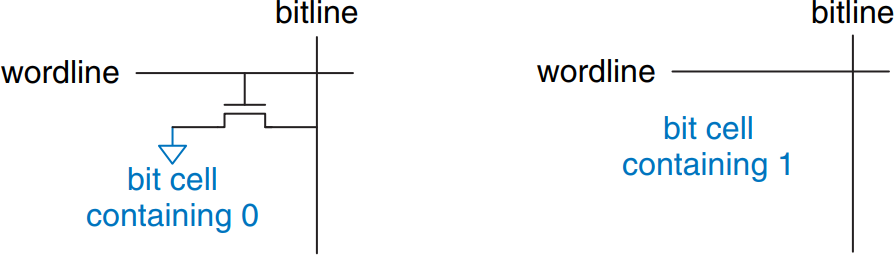
\includegraphics[width=0.6\textwidth]{rom_bit_cell.png}
    \caption{A ROM bit cell}
    \label{fig:rom_bit_cell}
  \end{figure}

  To read a cell, the bitline is \textit{weakly} pulled HIGH. Then, the wordline is turn ON. If the transistor is present, it pull the bitline LOW; otherwise, the bitline remains HIGH.

  Note that ROM is read only memory, and so there is no way to write to a bitcell.

  %%%%%%%%%%%%%%%%%%%%
  % Logic Using Memory Arrays
  %%%%%%%%%%%%%%%%%%%%
  \item \textbf{Logic Using Memory Arrays}

  Memory arrays can perform combinational logic functions despite their primary usage for data storage. Memory arrays used to perform logic are called \textit{lookup tables} (\textit{LUTs}). Using memory to perform logic, the user can look up the output value for a given input combination (address). Each address corresponds to a row in the truth table, and each data bit corresponds to an output value.
\end{enumerate}

%%%%%%%%%%%%%%%%%%%%%%%%%%%%%%%%%%%%%%%%
% Logic Arrays
%%%%%%%%%%%%%%%%%%%%%%%%%%%%%%%%%%%%%%%%
\subsection{Logic Arrays}

Like memory, gates can be organized into regular arrays called \textit{logic arrays}. These logic arrays can perform any function without the user having to connect wires in specific ways because they are made programmable. Most logic arrays are also configurable, which means the designer can modify them programmatically without replacing the hardware.

\begin{enumerate}
  %%%%%%%%%%%%%%%%%%%%
  % Programmable Logic Array
  %%%%%%%%%%%%%%%%%%%%
  \item \textbf{Programmable Logic Array}

  \textit{Programmable logic arrays} (\textit{PLAs}) implement two-level combinational logic in sum-of-products (SOP) forms. PLAs are built from an AND array followed by an OR array, as shown in Figure~\ref{fig:mnp_bit_pla}

  \begin{figure}[ht]
    \centering
    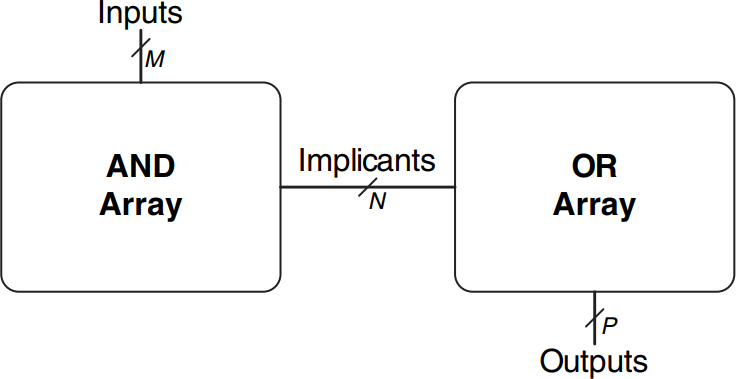
\includegraphics[width=0.5\textwidth]{mnp_bit_pla.png}
    \caption{A $M \times N \times P$-bit PLA}
    \label{fig:mnp_bit_pla}
  \end{figure}

  $M$ inputs drive an AND array, which produce $N$ implicants. The implicants then drive the OR array, which produces a $P$ outputs. A dot notation of a friendly example of a $3 \times 3 \times 2$-bit PLA is as follows:

  \newpage

  \begin{figure}[ht]
    \centering
    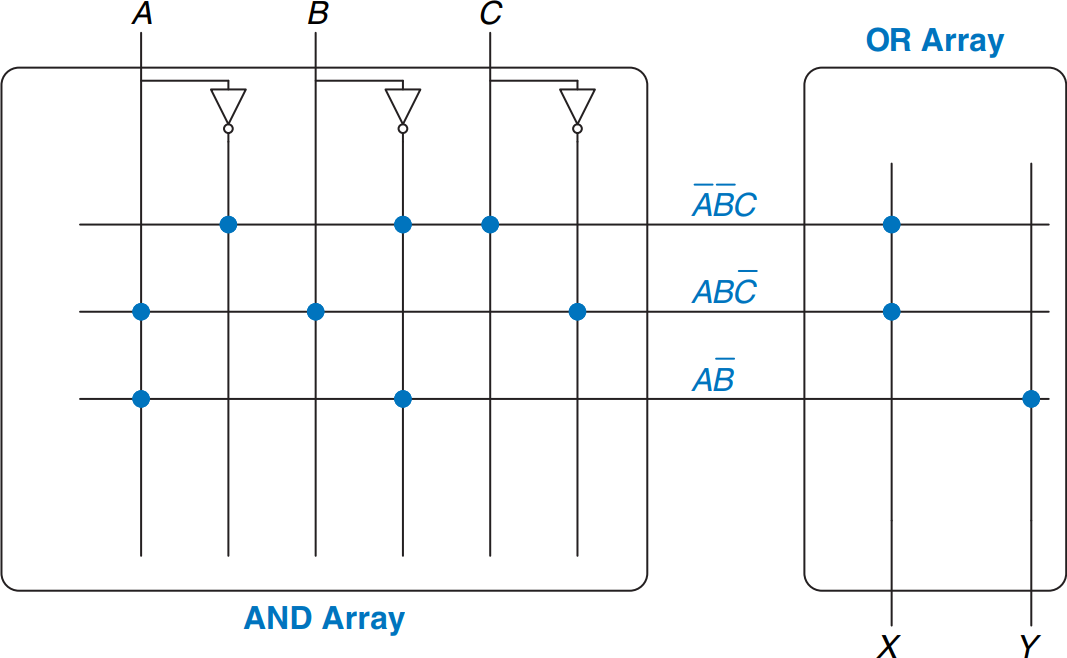
\includegraphics[width=0.5\textwidth]{3x3x2_pla.png}
  \end{figure}

  In this dot notation, each row of dots is an AND gate, and the dots on the corresponding row specifies the input to that AND gate.

  %%%%%%%%%%%%%%%%%%%%
  % Field Programmable Gate Array
  %%%%%%%%%%%%%%%%%%%%
  \item \textbf{Field Programmable Gate Array}

  Since PLAs are the older technology which can only perform combinational logic functions, the newer technology creates \textit{field programmable gate arrays} (\textit{FPGA}) which can perform both combinational logic and sequential logic. The logic gates of an FPGA are reconfigurable through software.

  The FPGAs are more powerful and flexible than PLAs for various reasons:

  \begin{itemize}
    \item Implement both combinational and sequential logic (versus only combinational logic functions for PLAs)
    \item Implement multilevel logic functions (versus two-level logic functions for PLAs)
    \item Built-in multipliers
    \item High-speed I/Os
    \item Data converters using analog-to-digital converters (ADC)
    \item Large RAM arrays
    \item Better processors.
  \end{itemize}

  FPGAs are built as an array of configurable \textit{logic elements} (\textit{LEs}), also referred to as \textit{configurable logic blocks} (\textit{CLBs}). Each LE can be configured to perform combinational and sequential logic. The LEs are surrounded by \textit{input/output elements} (\textit{IOEs}) for interfacing with the world.

  %%%%%%%%%%%%%%%%%%%%
  % Array Implementation
  %%%%%%%%%%%%%%%%%%%%
  \item \textbf{Array Implementation}

  To minimize the size and cost, ROMs and PLAs usually use pseudo-nMOS or dynamic circuits instead of conventional logic gates. For example, Figure~\ref{fig:rom_pseudo_nmos_implementation} compares the implementation of a ROM using the dot notation (conventional logic gate) with a pseudo-nMOS implementation:

  \newpage

  \begin{figure}[ht]
    \centering
    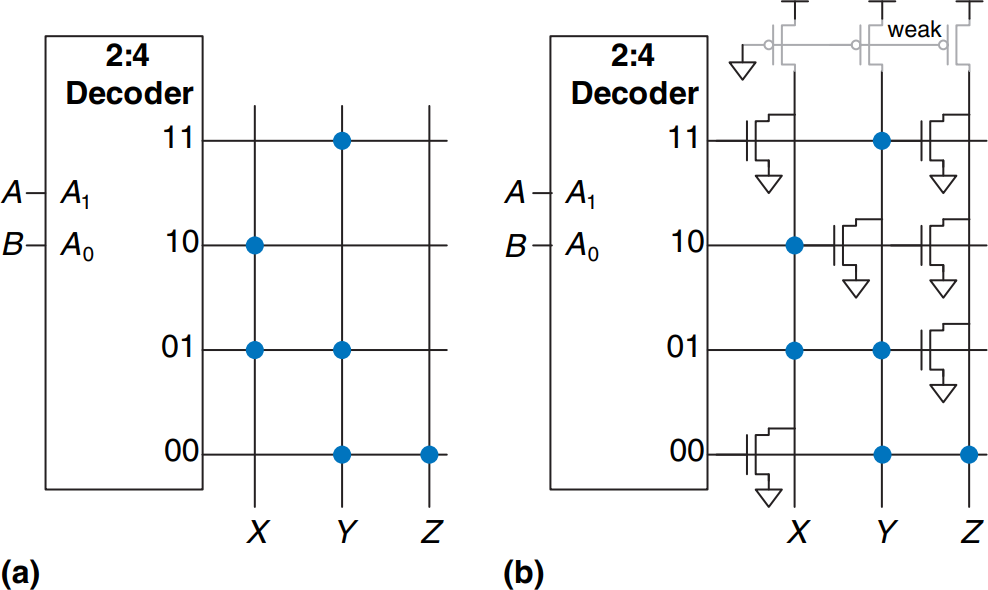
\includegraphics[width=0.5\textwidth]{rom_pseudo_nmos_implementation.png}
    \caption{ROM implementations: (a) dot notation, (b) pseudo-nMOS circuit}
    \label{fig:rom_pseudo_nmos_implementation}
  \end{figure}
\end{enumerate}

An nMOS transistor is placed at the junction without a dot in the array. Note that in pseudo-nMOS circuits, the weak pMOS transistor pulls the output HIGH \textit{only if} there is no path to GND through the pulldown (nMOS) network.

%%%%%%%%%%%%%%%%%%%%%%%%%%%%%%%%%%%%%%%%
% Summary
%%%%%%%%%%%%%%%%%%%%%%%%%%%%%%%%%%%%%%%%
\subsection{Summary}

%%%%%%%%%%%%%%%%%%%%%%%%%%%%%%%%%%%%%%%%%%%%%%%%%%%%%%%%%%%%%%%%%%%%%%%%%%%%%%%%
% Grey Box Exploration
%%%%%%%%%%%%%%%%%%%%%%%%%%%%%%%%%%%%%%%%%%%%%%%%%%%%%%%%%%%%%%%%%%%%%%%%%%%%%%%%
\section{Grey Box Exploration}

\begin{enumerate}
  %%%%%%%%%%%%%%%%%%%%%%%%%%%%%%%%%%%%%%%%
  % First grey box
  %%%%%%%%%%%%%%%%%%%%%%%%%%%%%%%%%%%%%%%%
  \item The first blurb is on page , which states \textit{}

  %%%%%%%%%%%%%%%%%%%%%%%%%%%%%%%%%%%%%%%%
  % Second grey box
  %%%%%%%%%%%%%%%%%%%%%%%%%%%%%%%%%%%%%%%%
  \item The second blurb is on page , which states \textit{}
\end{enumerate}

%%%%%%%%%%%%%%%%%%%%%%%%%%%%%%%%%%%%%%%%%%%%%%%%%%%%%%%%%%%%%%%%%%%%%%%%%%%%%%%%
% Figures
%%%%%%%%%%%%%%%%%%%%%%%%%%%%%%%%%%%%%%%%%%%%%%%%%%%%%%%%%%%%%%%%%%%%%%%%%%%%%%%%
\section{Figures}

Two figures were selected from this chapter for special recognition. Figure was selected because

% \begin{figure}[ht]
%     \centering
%     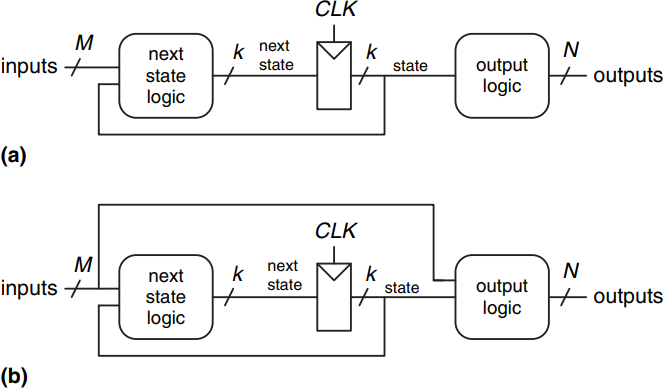
\includegraphics[width=0.5\textwidth]{moore_and_mealy_fsm.png}
%     \caption{Finite state machines: (a) Moore machine, (b) Mealy machine}
%     \label{fig:13}
% \end{figure}

Figure was selected because

% \begin{figure}[ht]
%     \centering
%     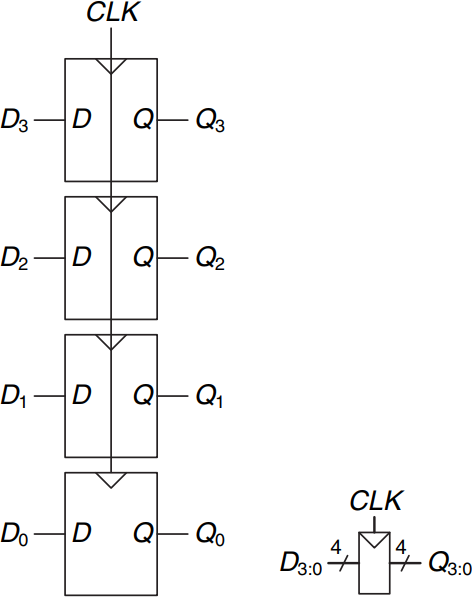
\includegraphics[width=0.25\textwidth]{register_4bit.png}
%     \caption{Inside of a 4-bit register}
%     \label{fig:14}
% \end{figure}

%%%%%%%%%%%%%%%%%%%%%%%%%%%%%%%%%%%%%%%%%%%%%%%%%%%%%%%%%%%%%%%%%%%%%%%%%%%%%%%%
% Example Problems
%%%%%%%%%%%%%%%%%%%%%%%%%%%%%%%%%%%%%%%%%%%%%%%%%%%%%%%%%%%%%%%%%%%%%%%%%%%%%%%%
\section{Example Problems}

See the attached images on the next four pages.

% 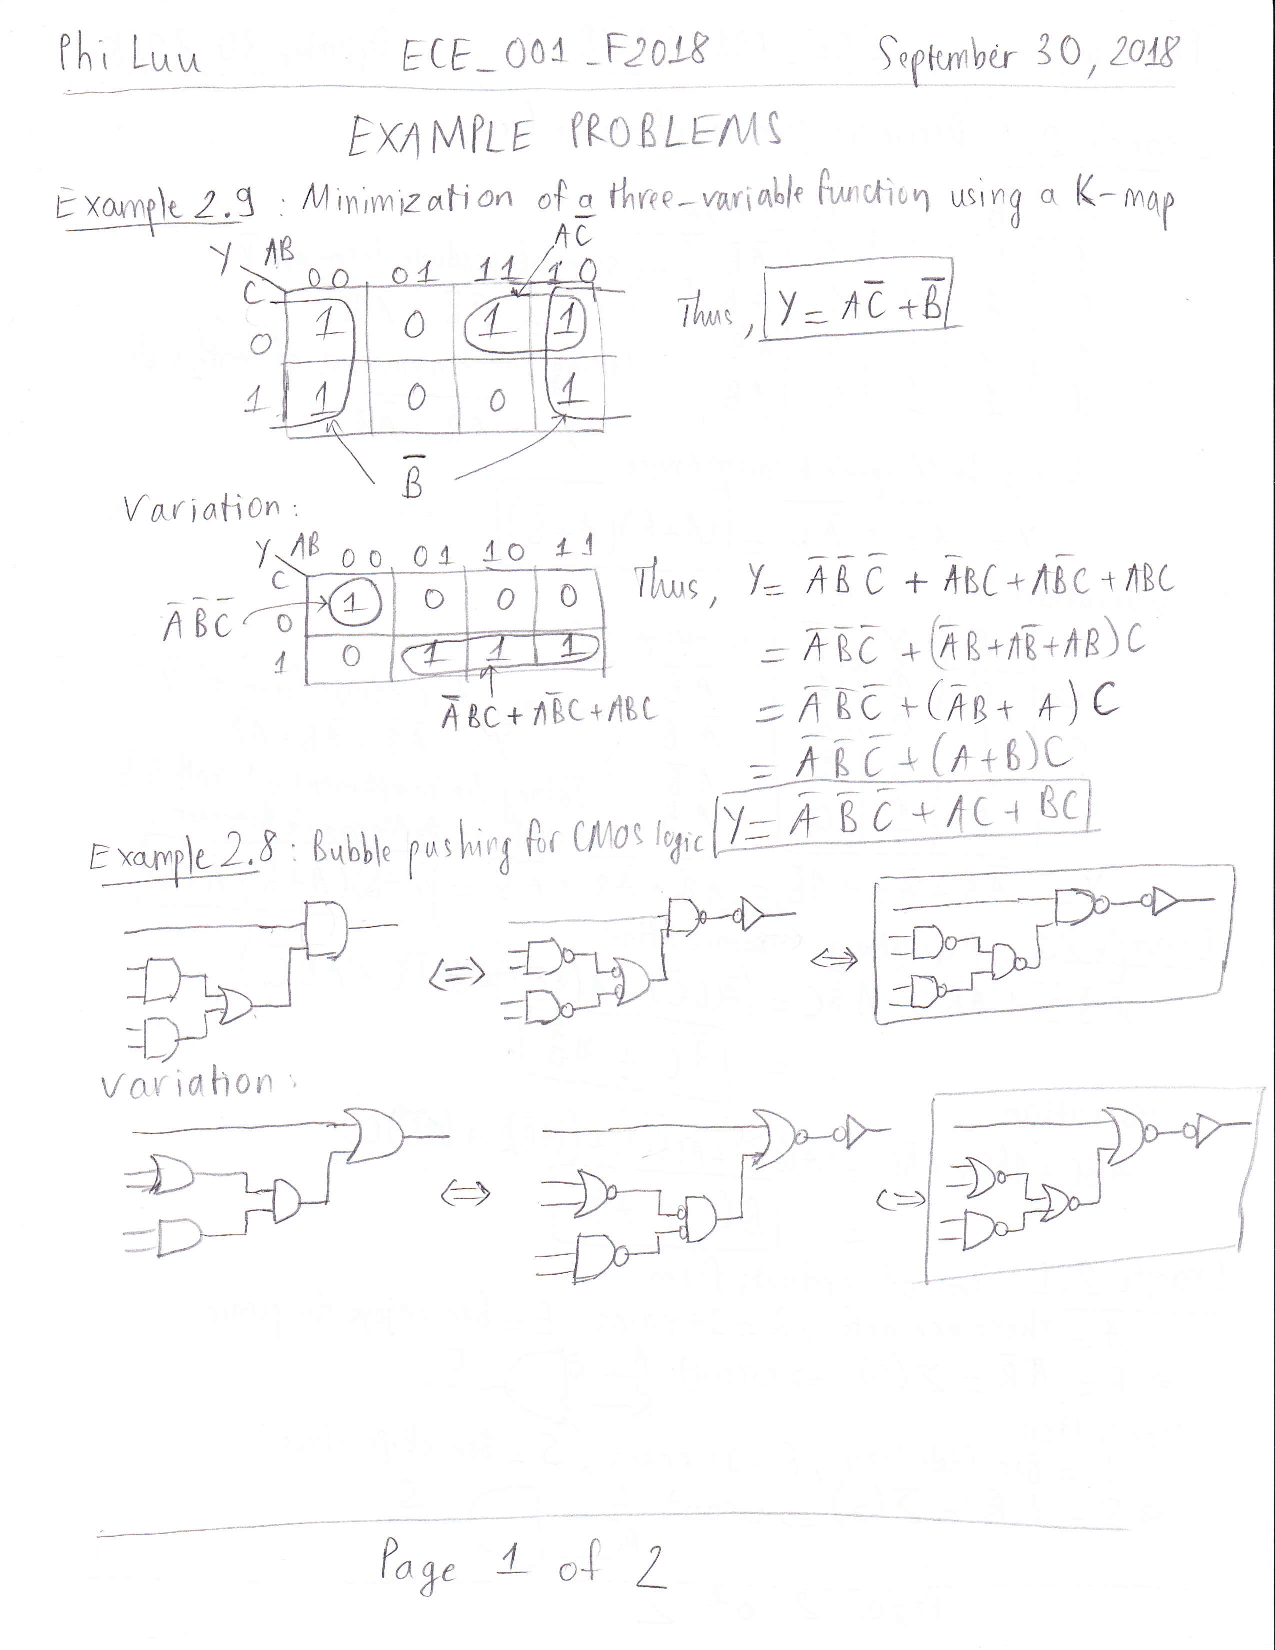
\includepdf[page=-]{example_problems}

%%%%%%%%%%%%%%%%%%%%%%%%%%%%%%%%%%%%%%%%%%%%%%%%%%%%%%%%%%%%%%%%%%%%%%%%%%%%%%%%
% Glossary
%%%%%%%%%%%%%%%%%%%%%%%%%%%%%%%%%%%%%%%%%%%%%%%%%%%%%%%%%%%%%%%%%%%%%%%%%%%%%%%%
\section{Glossary}

All definitions were found from the Google search engine, typing "define arithmetic logic unit" for the first item.

\begin{enumerate}
  \item Arithmetic Logic Unit (ALU)

  noun:

  \begin{enumerate}
    \item A unit in a computer that carries out arithmetic and logical operations.
  \end{enumerate}

  \item Comparator

  noun:

  \begin{enumerate}
    \item a device for comparing a measurable property or thing with a reference or standard.

    \begin{itemize}
      \item an electronic circuit for comparing two electrical signals.
      \item something used as a standard for comparison.
    \end{itemize}
  \end{enumerate}

  \item{Read Only Memory}

  noun:

  \begin{enumerate}
    \item {[computing]} memory read at high speed but not capable of being changed by program instructions.
  \end{enumerate}

  \item{Array}

  noun:

  \begin{enumerate}
    \item an impressive display or range of a particular type of thing.

    \item an ordered series or arrangement.
      \begin{itemize}
        \item an arrangement of troops.
        \item {[mathematics]} an arrangement of quantities or symbols in rows and columns; a matrix.
        \item {[computing]} an indexed set of related elements.
      \end{itemize}

    \item {[literary]} elaborate or beautiful clothing.
    \item {[law]} a list of jurors empaneled.
  \end{enumerate}

  verb:

  \begin{enumerate}
    \item display or arrange (things) in a particular way.
    \item dress someone in (the clothes specified).
    \item {[law]} empanel (a jury).
  \end{enumerate}

  \item{Random Access}

  noun:

  \begin{enumerate}
    \item {[computing]} the process of transferring information to or from memory in which every memory location can be accessed directly rather than being accessed in a fixed sequence.
  \end{enumerate}
\end{enumerate}

%%%%%%%%%%%%%%%%%%%%%%%%%%%%%%%%%%%%%%%%%%%%%%%%%%%%%%%%%%%%%%%%%%%%%%%%%%%%%%%%
% Interview Question
%%%%%%%%%%%%%%%%%%%%%%%%%%%%%%%%%%%%%%%%%%%%%%%%%%%%%%%%%%%%%%%%%%%%%%%%%%%%%%%%
\section{Interview Question}

See the attached image on the next page.

% 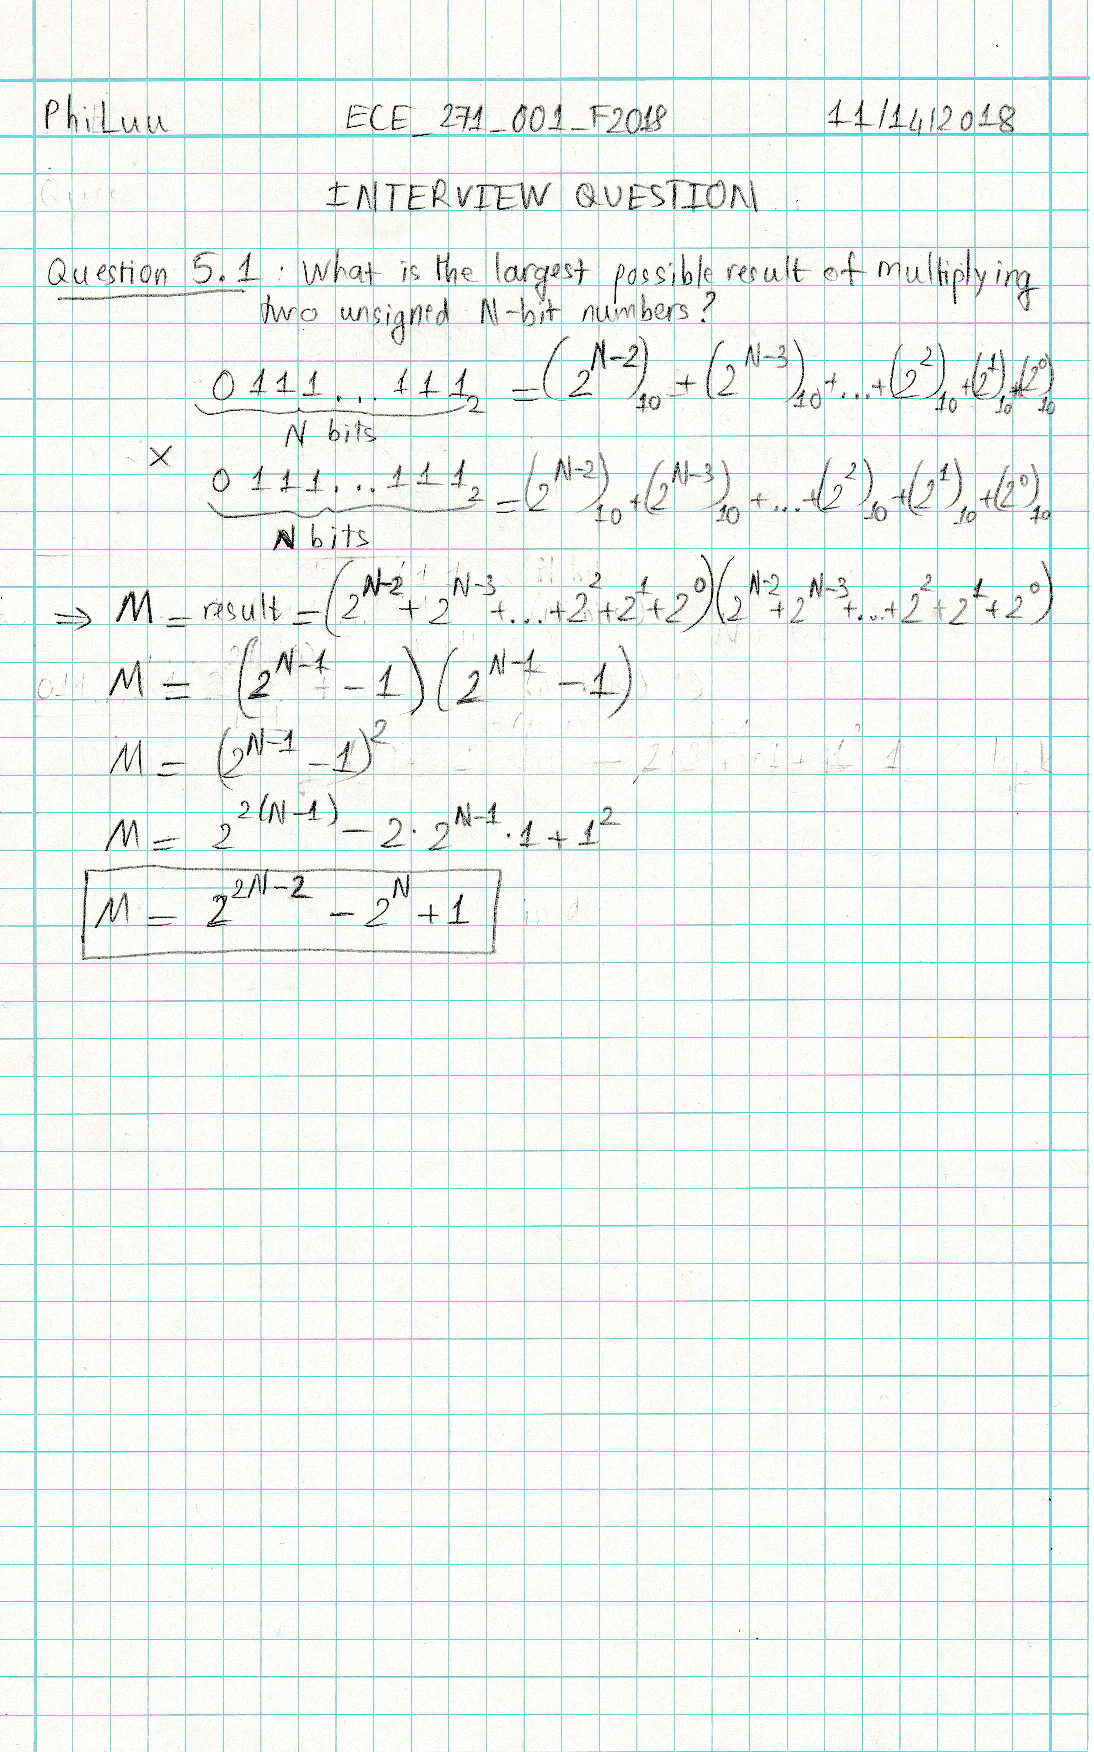
\includepdf[page=-]{interview_question}

%%%%%%%%%%%%%%%%%%%%%%%%%%%%%%%%%%%%%%%%%%%%%%%%%%%%%%%%%%%%%%%%%%%%%%%%%%%%%%%%
% Reflection
%%%%%%%%%%%%%%%%%%%%%%%%%%%%%%%%%%%%%%%%%%%%%%%%%%%%%%%%%%%%%%%%%%%%%%%%%%%%%%%%
\section{Reflection}

%%%%%%%%%%%%%%%%%%%%%%%%%%%%%%%%%%%%%%%%%%%%%%%%%%%%%%%%%%%%%%%%%%%%%%%%%%%%%%%%
% Questions for Lecture
%%%%%%%%%%%%%%%%%%%%%%%%%%%%%%%%%%%%%%%%%%%%%%%%%%%%%%%%%%%%%%%%%%%%%%%%%%%%%%%%
\section{Questions for Lecture}

\begin{enumerate}
  \item
  \item
  \item
\end{enumerate}

\end{document}
